\PassOptionsToPackage{table}{xcolor}
\documentclass[nobib,nofonts]{tufte-handout}

%\geometry{showframe} % display margins for debugging page layout

%%% MF additions
% \usepackage[table]{xcolor}
\usepackage[nographicx, nohyperref, nosubcaption, nogb4e, nobiblatex]{../99-auxiliary-files/00-mypackages}
\usepackage{../99-auxiliary-files/00-mycommands}
\usepackage{../99-auxiliary-files/00-myenvironments}

\usepackage{titlesec}
\usepackage{etoolbox}
\usepackage{tikz-qtree}
\usepackage{subcaption}

% \titleformat{\section}
% {\large\bfshape}{\thesection}{1em}{}

\setcounter{secnumdepth}{5}
\renewcommand\thesection{\arabic{section}}

% this length controls tha hanging indent for titles
% change the value according to your needs
\newlength\titleindent
\setlength\titleindent{0.7cm}

\pretocmd{\paragraph}{\stepcounter{subsection}}{}{}
\pretocmd{\subparagraph}{\stepcounter{subsubsection}}{}{}

\titleformat{\chapter}[block]
  {\normalfont\huge\bfseries}{}{0pt}{\hspace*{-\titleindent}}

\titleformat{\section}
  {\normalfont\Large\itshape}{\llap{\parbox{\titleindent}{\thesection\hfill}}}{0em}{}

\titleformat{\subsection}
  {\normalfont\itshape}{\llap{\parbox{\titleindent}{\thesubsection\hfill}}}{0em}{}

\titleformat{\subsubsection}
  {\normalfont\normalsize\itshape}{\llap{\parbox{\titleindent}{\thesubsubsection}}}{0em}{}

\titleformat{\paragraph}[runin]
  {\normalfont\normalsize\itshape}{}{-0.7cm}{}[\xspace \ \ \ \ ]

\titleformat{\subparagraph}[runin]
  {\normalfont\normalsize}{\llap{\parbox{\titleindent}{\thesubsubsection\hfill}}}{0em}{}

\titlespacing*{\chapter}{0pt}{0pt}{20pt}
\titlespacing*{\subsubsection}{0pt}{3.25ex plus 1ex minus .2ex}{1.5ex plus .2ex}
\titlespacing*{\paragraph}{0pt}{3.25ex plus 1ex minus .2ex}{0em}
\titlespacing*{\subparagraph}{0pt}{3.25ex plus 1ex minus .2ex}{0em}

\DefineNamedColor{named}{mygray2}{cmyk}{0.55,0.25,0.25,0.25}
\newcommand{\mygray}[1]{\textcolor{mygray2}{#1}}

%%% Tufte style
\usepackage{graphicx} % allow embedded images
  \setkeys{Gin}{width=\linewidth,totalheight=\textheight,keepaspectratio}
  \graphicspath{{graphics/}} % set of paths to search for images

\usepackage{fancyvrb} % extended verbatim environments
  \fvset{fontsize=\normalsize}% default font size for fancy-verbatim environments

% Standardize command font styles and environments
\newcommand{\doccmd}[1]{\texttt{\textbackslash#1}}% command name -- adds backslash automatically
\newcommand{\docopt}[1]{\ensuremath{\langle}\textrm{\textit{#1}}\ensuremath{\rangle}}% optional command argument
\newcommand{\docarg}[1]{\textrm{\textit{#1}}}% (required) command argument
\newcommand{\docenv}[1]{\textsf{#1}}% environment name
\newcommand{\docpkg}[1]{\texttt{#1}}% package name
\newcommand{\doccls}[1]{\texttt{#1}}% document class name
\newcommand{\docclsopt}[1]{\texttt{#1}}% document class option name
\newenvironment{docspec}{\begin{quote}\noindent}{\end{quote}}% command specification environment

\newcommand{\proplog}{\acro{PropLog}}
\newcommand{\predlog}{\acro{PredLog}}
\newcommand{\EFSQ}{\ensuremath{\mathit{EFSQ}}\xspace}

%%%%%%%%%%%%%%%%%%%%%%%%%%%%%%%%%%%%%%%%%%%%%%%%%%

% \usepackage[sc,osf]{mathpazo}
% \linespread{1.05}



\title{Predicate Logic}

\author[M.~Franke]{Michael Franke}

\date{} % without \date command, current date is supplied

\begin{document}

\maketitle

\begin{abstract}
\noindent
Formulas of predicate logic;
predicate letters, variables \& individual constants;
domain of quantification;
quantifier scope and binding;
atomic sentences;
predicate-logical meaning of natural language sentences;
semantics of predicate logic;
\end{abstract}

\section{Motivation}

We can think of propositional logic as a system that formalizes the meaning of important functional terms, namely the sentential connectives (negation, conjunction, disjunction, implication).
This carries a long way towards capturing what sound logical inference is.
But it also fails to capture crucial patterns of inference.
For example, if we know that
\begin{quote}
  Alex is as tall as Bo
\end{quote}
we also know that
\begin{quote}
  Bo is as tall as Alex
\end{quote}
in virtue of our knowledge of what the predicate ``being as tall as'' means.
Propositional logic cannot capture this.
It can model the first sentences as $p$ (= ``Alex is as tall as Bo'') and the second as $q$ (= ``Bo is as tall as Alex''), but since we cannot look inside the structure of a simple proposition, there is no way in which we can say that $p$, based on its internal form and relatedness to the internal form of $q$, must necessarily entail $q$.\sidenote{We can, of course, make the additional premise by writing down that $p \rightarrow q$, but that clearly does not explain the general relationship.}

Predicate logic (\predlog) is an extension of \proplog which adds two things.
Firstly, \predlog models the internal structure of atomic propositions in terms of \emph{predicates} and \emph{individual constants}.
For example, we could have a (two-place) predicate $T$ meaning (``being as tall as'') and two symbols, so-called individual constants, $a$ and $b$ which represent Alex and Bo respectively.
We can then translate the sentence ``Alex is as tall as Bo'' into the formula $Tab$, which is a minimal truth-evaluable unit, but does have internal structure.
Similarly, the sentence ``Bo is as tall as Alex'' would translate into $Tba$.

Secondly, \predlog allows to capture \emph{quantification}, which is extremely important in order to capture general rules, generalizations and key aspects of our semantic and world knowledge.\sidenote{Semantic knowledge is what we know about the meaning of words and expressions. For example, semantic knowledge tells us that ``being taller than'' is a transitive relation, and that ``being as tall as'' is an equivalence relation. World knowledge is what we know about the world. For example, we know that Berlin is the capital of Germany.}
Imagine that you have a reasoning machine (computer, robot, friend \dots) able to compute logical inferences in predicate logic.
Even though we have not introduced any of the formal machinery (syntax, semantics, definition of validity, deduction system) necessary to make such formal reasoning precise, imagine you give this machine the information $Tab$.
You want it to represent ``Alex is as tall as Bo,'' but the machine only has the string of symbols to work with.
Would that machine be able to conclude that $Tba$?
No, it wouldn't because it doesn't know that you want the symbol $T$ to mean ``being as tall as'' and not ``being taller than'' or anything else.
But, using predicate logic, you \emph{can} tell the system about the fundamental structural properties of the relation ``being as tall as,'' such as that it is reflexive.
In other words, you can express that ``being as tall as'' is a symmetric predict directly in \predlog with the formula:
\begin{align*}
 \forall x \myts \forall y \myts (Txy \rightarrow Tyx)
\end{align*}
which can be read as ``for all objects $x$ and $y$, if $x$ stands in relation $T$ to $y$, then so does $y$ to $x$.''
This formulas uses the quantifier \(\forall\) to express a generalization: something that holds of any pair of objects.
Generalizations of this kind are essential for human reasoning and \predlog captures the most basic aspects of quantification in a system of logical reasoning.
To be clear, the inference schema:
\begin{align*}
 Tab, \forall x \myts \forall y \myts (Txy \rightarrow Tyx) / Tba
\end{align*}
is logically valid in \predlog, but the schema:
\begin{align*}
 Tab / Tba
\end{align*}
is not.

\section{The language of predicate logic}

\subsection{Basic ingredients of predicate-logical formulas}

The formulas of \predlog consist:
\begin{multicols}{2}
\begin{itemize}
  \item individual constants $a,b,c, \dots, v$
  \item predicate letters $A, B, C, D \dots$
  \item variables $w, x,y,z$
  \item parentheses ( \ \ )
  \item sentential connectives $\neg, \wedge, \vee, \rightarrow, \leftrightarrow$
  \item quantifiers $\exists, \forall$
\end{itemize}
\end{multicols}
\emph{Individual constants} are denoted by lower-case Roman letters ($a, b, c, \dots, v $) up to $v$.\sidenote{If need be, we can also use indices like $a_{1}$, $a_{2}$ etc. This also holds for variables and predicate letters.}
Individual constants are like proper names: they refer to exactly one individual.
For example, the individual constant $a$ may be interpreted as referring to Alex and $b$ as referring to Bo.
Individuals in the sense of predicate logic need not be humans or animals. An individual is any kind of entity that can have properties or stand in some kind of relation to any other property. For example, constant $m$ may denote a particular copy of \emph{Moby Dick}.

\emph{Predicate letters} are denoted with upper-case Roman letters ($A, B, C, D \dots$).
Predicate letters will be used to denote properties or relations.
Each predicate letter has a unique \emph{arity}.
The arity of a predicate letter is always an integer bigger than zero.
It gives the number of elements that the predicate letter expects as an argument.
A predicate letter with arity one is also called \emph{unary} predicate letter and will be interpreted to refer to a property.
For example, if $B$ is a unary predicate letter denoting the property ``$x$ is a book'', then the expression $Bm$ can be interpreted as expressing that \emph{Moby Dick} is a book.
A predicate letter with arity bigger than one will be interpreted to denote a relation.
For example, if the predicate letter $L$ has arity two, it may stand for a two-place relations such as ``$x$ loves $y$''.
Consequently, we expect $L$ to have two arguments, so that $Lab$, $Lam$ or $Lmb$ would be well-formed expressions (no matter whether true or meaningful), while $Labm$, $Laaaa$ or $Lb$ would not be.

\emph{Variables} are denoted by lower-case Roman letters ($w, x,y,z$), starting from $w$.
Variables are only interpretable in the \emph{scope} of a quantifier, an important technical concept we will introduce later.
As a first intuitive guide, think of variables as similar to pronouns\sidenote{A proper logical treatment of pronouns in natural language requires more sophisticated logical systems, like \emph{dynamic logics} or \emph{discourse representation theory}.} which are used to refer to an unnamed individual introduced by a quantifying expression like in these examples:

\begin{quote}
For every boy it holds that \emph{he} \dots \hfill \mygray{[\emph{he} = some boy]}\\
There is a boy for which it holds that \emph{he} \dots \hfill \mygray{[\emph{he} = some boy]}\\
\end{quote}

To build formulas, \predlog also uses \emph{parentheses} and exactly the same \emph{sentential connectives} as \proplog does.

\emph{Quantifiers} are special functional elements of the language of \predlog.
The quantifier $\exists$ is the \emph{existential quantifier}.
It is read as ``there is'' or ``there exists.''
For example, the formula $\exists x (Bx \wedge Ix)$ would be read as ``there is an $x$ such that $x$ has property $B$ and $I$.''
It would mean that there is an individual which has the property denoted by $B$ (e.g., it is a book) and the property denoted by $I$ (e.g., it is interesting).
In short, this formula would express that there is at least one interesting book.
The quantifier $\forall$ is the \emph{universal quantifier}.
It is read as ``for all,'' ``all'' or ``every.''
For example, the formula $\forall x (Bx \rightarrow Ix)$ would be read as ``for all $x$ it holds that if $x$ has property $B$, then it also has property $I$.''
This would express that all books are interesting.

\subsection{Formulas}

The language $\mathfrak{L}$ of \predlog is the set of all \emph{formulas} which are recursively defined as follows:

\begin{enumerate}[(i)]
  \item If $A$ is an $n$-ary predicate letter and if $t_1, \dots, t_n$ are individual constants     or variables, then $At_1 \dots t_n$ is a formula.
  \item If $\varphi$ is a formula, then so is $\neg \varphi$.
  \item If $\varphi$ and $\psi$ are formulas, so are:\sidenote{We allow ourselves to omit the outermost pair of parentheses as in \proplog.}
    \vspace*{-0.4cm}
    \begin{multicols}{4}
      \begin{enumerate}[a.]
        \item ($\varphi \wedge \psi$)
        \item ($\varphi \vee \psi$)
        \item ($\varphi \rightarrow \psi$)
        \item ($\varphi \leftrightarrow \psi$)
      \end{enumerate}
    \end{multicols}
    \vspace*{-0.4cm}
  \item If $\varphi$ is a formula and if $x$ is a variable, then these are formulas:
    \vspace*{-0.4cm}
    \begin{multicols}{2}
      \begin{enumerate}[a.]
        \item $\forall x \myts \varphi$ \ \ \ [\emph{universal statement}]
        \item $\exists x \myts \varphi$ \ \ \ [\emph{existential statement}]
      \end{enumerate}
    \end{multicols}
    \vspace*{-0.4cm}
  \item Anything that cannot be constructed by (i)--(iv) is not a formula.
\end{enumerate}

Here are examples of formulas of \predlog, together with intuitive paraphrases based on the interpretation that $a$ is Alex, $b$ is Bo, $m$ is the book \emph{Moby Dick}, $Lxy$ means ``$x$ likes $y$,'' $Bx$ means ``$x$ is a book'' and $Oxy$ means that ``$x$ owns $y$.''
\begin{align*}
  & Lam                           && \text{Alex likes Moby Dick.} \\
  & Lab \wedge Lba                && \text{Alex likes Bo and Bo likes Alex.} \\
  & \neg Oba                && \text{Bo does not own Alex.} \\
  & \exists x (Bx \wedge Oax)                && \text{Alex owns a book.} \\
  & \forall x \myts ((Bx \wedge Obx) \rightarrow  Lax) && \text{Alex likes every book Bo owns.} \\
  & \neg \exists x \myts (Bx \wedge Oax) && \text{Alex does not own any books.} \\
  & \forall x \myts (Bx \rightarrow \neg Oax) && \text{Alex does not own any books.}
\end{align*}

\subsection{Syntactic trees}

The recursive definition for formulas of \predlog gives an internal structure to each formula which we can represent using \emph{syntactic trees}, just like for \proplog.
For \predlog the syntactic structure of a formula is particularly important for the important concept of the \emph{scope of a quantifier} and the crucial notion of \emph{variable binding} (see below).
The syntactic structure, and with it the scope of a quantifier, depends on proper use of parentheses.

To illustrate, assume that we want to explicate the logical structure of the sentence:
\begin{quote}
  Alex owns a book.
\end{quote}
Here are two candidate formulas, of which the left one is correct, the right one incorrect:
\begin{align*}
 & \exists x \myts (Bx \wedge Oax) && \exists x \myts Bx \wedge Oax
\end{align*}
A paraphrase of the second (incorrect) formula is, roughly: ``There is a book and Alex owns them, him, her, it.''
The point is that in the second formula the $x$ might but need not refer to the book, because it is not part of the formula ``dominated by \(\exists\),'' so to speak.
This shows in the different syntactic trees.

\begin{center}
  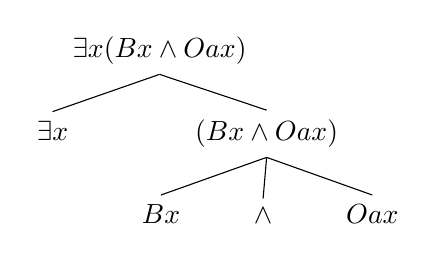
\begin{tikzpicture}[sibling distance=20pt, level distance=30pt]
    \Tree [.{$\exists x \myts (Bx \wedge Oax)$} [. $\exists x$ ] [. {$(Bx \wedge Oax)$} [. $Bx$ ] [. $\wedge$ ] [. $Oax$ ] ] ]
  \end{tikzpicture}
  \hfill
    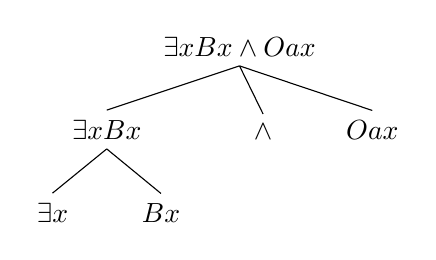
\begin{tikzpicture}[sibling distance=20pt, level distance=30pt]
    \Tree [.{$\exists x \myts Bx \wedge Oax$} [. {$\exists x \myts Bx$} [. $\exists x$ ] [. $Bx$ ] ] [. {$\wedge$} ] [. $Oax$ ] ]
  \end{tikzpicture}
\end{center}

\subsection{Terminology}

Just like in \proplog, formulas of \predlog can be named by their main operator.
For example, the following formulas can be called \emph{conjunctions}:\sidenote{The second example here expresses the idea that Alex owns a book, and that Alex likes a book, where these could be the same or different books.}
\begin{align*}
  & Oam \wedge Lam && \exists x \myts (Bx \wedge Oax) \wedge \exists x \myts (Bx \wedge Lax)
\end{align*}
A formula whose main operator is a universal quantifier can be called a \emph{universal formula} or a \emph{universal statement}; a formula whose main operator is an existential quantifier can be called an \emph{existential formula} or an \emph{existential statement}.
For example, the formula $\exists x \myts (Bx \wedge Oax)$ from above is an existential statement, but the formula $\exists x \myts Bx \wedge Oax$ is a conjunction (as evidenced by the syntactic trees given above).

If $A$ is an $n$-ary predicate letter and if $t_1, \dots, t_n$ are individual constants, then $At_1 \dots t_n$ is an \markdef{atomic sentence}.
Atomic sentences are minimal truth-evaluable units of the language of \predlog, akin to the proposition letters of \proplog.

\section{Quantifier scope \& binding}

Not every well-formed formula of \predlog is interpretable.
Consider the formula $Lax$.
We might paraphrase this as ``Alex likes them, us, him, her or it.''
Without knowing what $x$ refers to, this formula ---though a formula of \predlog--- is not interpretable.
We therefore introduce terminology to speak about which occurrences of variables are interpretable, which are not, and how a variable that is interpretable is to be interpreted.
The relevant technical terms are \emph{scope}, as well as \emph{bound} and \emph{free} occurrences of a variable.

If $\forall x \myts \psi$ is a subformula of $\varphi$, then $\psi$ is the \emph{scope} of this occurrence of the quantifier $\forall x$ in $\varphi$. The same holds for $\exists x$.
An occurrence of a variable $x$ in a formula $\varphi$ (in a place where also an individual constant could appear, so not the $x$ in ``$\forall x$'' and ``$\exists x$''), is \emph{free} in $\varphi$ if $x$ is not in the scope of a quantifier $\forall x$ or $\exists x$.
If $\forall x \myts \psi$ (or $\exists x \myts \psi$) is a subformula of $\varphi$ and if an occurrence of $x$ is free in $\psi$, then this occurrence of $x$ is \emph{bound} by the quantifier $\forall x$ (or $\exists x$).

Here are examples:\sidenote{The last formula is well-formed and interpretable, but not very cooperative for an interpreter. In practice, we would rather like to write $\exists x (\myts Px \wedge \forall y \myts Qy)$}
\begin{align*}
  & Px && \text{$x$ is free} \\
  & Px \wedge \forall x \myts Qx && \text{the first occurrence of $x$ is free, the second bound} \\
  & \exists x (\myts Px \wedge Qx) && \text{both occurrences of $x$ are existentially bound}\\
  & \exists x \myts Px \wedge \forall x \myts Qx && \text{first occur.~existentially bound, second universally bound}\\
  & \exists x (\myts Px \wedge \forall \myts x Qx) && \text{first occur.~existentially bound, second universally bound}
\end{align*}

\section{Domain of quantification}

Even if all variables in a formula are bound, in order to be able to interpret ---even if only intuitively--- what a formula of \predlog could mean, we need information about the \emph{domain of quantification} $D$.
Take the formula $\forall x \myts (Lxa)$ with the interpretation of $a$ and $Lxy$ as before.
We might take this to mean that everybody likes Alex, or that everything on earth (including the book \emph{Moby Dick}) likes Alex.
So, when we write down a formula with quantifiers in \predlog, it will only be interpretable if we specify which individuals the quantification should range over.
We call this the \emph{domain of quantification} $D$.
Remember that you must always specify the domain of quantification $D$ in translation exercises or other applications where your formulas are supposed to be meaningfully interpretable.

\section{Translations from natural langauge to \predlog}

Just like \proplog, \predlog is useful for uncovering the logical structure of sentences.
Unlike \proplog, \predlog can lay bare the internal structure of atomic propositions and aspects of quantification.

Suppose we want to translate this sentences to predicate logic:
\begin{quote}
Alex likes Bo but if Bo likes Alex, Bo likes everyone.
\end{quote}

A formula that captures the logical structure of this sentence is:
\begin{align*}
  Lab \wedge (Lba \rightarrow \forall x \myts Lbx)
\end{align*}
Such a translation is only complete, strictly speaking, when we also explicitly state the \emph{translation key}, which defines what each individual constant and predicate letter refers to, as well as the arity of each predicate letter.
In the example at hand, the translation key would be:\sidenote{Notice that the arity of the predicate $L$ is fixed by the notation $Lxy$ and that it is crucial for the translation key to specify exactly what a predicate like $L$ means, i.e., is first argument the slot for the person doing or receiving the liking?}
\begin{enumerate}[(i)]
  \item $a$: Alex
  \item $b$: Bo
  \item $Lxy$: $x$ likes $y$
\end{enumerate}
The domain of quantification should be the set of all human beings.
If the domain of quantification should also include non-humans, we would have to adapt the formula:
\begin{align*}
  Lab \wedge (Lba \rightarrow \forall x \myts (Hx \rightarrow Lbx))
\end{align*}
and also include the predicate letter $H$ in the translation key like so:
\begin{enumerate}[(iv)]
  \item $Hx$: $x$ is a human being
\end{enumerate}

\bigskip
\noindent \colorbox{mygray}{\centering
  \begin{minipage}{1.0\textwidth}

    \begin{exercise}
      For each of the following strings, determine whether they are formulas of \predlog or not. Assume that $P$ and $Q$ are unary predicate letters, and that $R$ is a binary predicate letter.
      \begin{multicols}{2}
      \begin{enumerate}[(i)]
        \item $Px \rightarrow \exists \myts x$
        \item $\forall x (Px)$
        \item $\forall x Px$
        \item $(\forall x Px)$
        \item $Px \vee \exists \myts x Px$
        \item $\forall y Px \vee \exists \myts x Px$
        \item $\forall y (Rxy \vee \exists \myts x Px)$
        \item $\forall y (Rxy \vee \exists \myts x Px)$
      \end{enumerate}
    \end{multicols}
    \end{exercise}

    \begin{exercise}
      For each of the following formulas of predicate logic, determine whether each occurrence of a variable is a free or bound occurrence. If it is a bound occurrence, determine which quantifier binds it.
      \begin{multicols}{2}
      \begin{enumerate}[(i)]
        \item $Px$
        \item $\exists x \myts Lxj$
        \item $\exists x \myts Lxy$
        \item $\exists x \myts Px \wedge Lxj$
        \item $\exists x \myts (Px \wedge Lxj)$
        \item $\exists x \myts (Px \wedge \forall x \myts Lxj)$
      \end{enumerate}
    \end{multicols}
    \end{exercise}

    \begin{exercise}
      Translate the following sentences into the language of predicate logic. Preserve as much of   the logical structure as possible and give the translation key and the domain of   quantification (here: $D: \text{people}$).
      \begin{enumerate}[(i)]
        \item Everybody is friendly.
        \item Everybody loves somebody.
        \item Every pilot loves Bill.
        \item If Mary is a pilot, someone loves her.
        \item Every pilot is unfriendly.
        \item Some pilots are friendly.
        \item No pilot is friendly.
        \item Nobody loves anyone who is in love with a pilot.
      \end{enumerate}
    \end{exercise}
  \end{minipage}
}


\end{document}
